% AI Algebra Tutor -- MSCS capstone report (about 8 pages).
% Compile with pdfLaTeX + BibTeX (Overleaf default).
% A longer version with more implementation detail is in report/report.md.
\documentclass[11pt]{article}

\usepackage[margin=1in]{geometry}
\usepackage[T1]{fontenc}
\usepackage[utf8]{inputenc}
\usepackage{lmodern}
\usepackage{microtype}
\usepackage{amsmath,amssymb}
\usepackage{booktabs}
\usepackage{tabularx}
\usepackage{graphicx}
\usepackage{subcaption}
\usepackage{enumitem}
\usepackage{xcolor}
\usepackage{tikz}
\usetikzlibrary{positioning,arrows.meta,fit,backgrounds}
\usepackage[numbers,sort&compress]{natbib}
\usepackage[colorlinks=true,linkcolor=blue!50!black,citecolor=blue!50!black,urlcolor=blue!50!black]{hyperref}

\setlist{itemsep=1pt,topsep=3pt}
\newcommand{\code}[1]{\texttt{#1}}
% Marks text the author still has to write. Remove before submitting.
\newcommand{\todo}[1]{\textcolor{red}{\textbf{[TODO:} #1\textbf{]}}}

\title{\textbf{AI Algebra Tutor: Adaptive Practice with Deep Knowledge Tracing and Verified LLM Feedback}\\[4pt]
\large MSCS Capstone Report}
\author{Mingqi Zhao\\[2pt] \small Advisor: Bolei Zhou}
\date{November 14, 2026}

\begin{document}
\maketitle

\begin{abstract}
Large language models (LLMs) can explain mathematics fluently, but they make errors and readily reveal answers, two failure modes that are harmful in tutoring. This project builds an adaptive algebra tutor that combines a Deep Knowledge Tracing (DKT) model of each student's mastery, a prerequisite-aware rule that recommends the next problem, and LLM-generated hints and explanations whose every mathematical step is verified with the SymPy computer algebra system before a student sees it. On ASSISTments 2009 data split by student, DKT reaches a test AUC of 0.751 versus 0.708 for Bayesian Knowledge Tracing (BKT). In a paired experiment on 127 hints, verification reduced a smaller LLM's answer-leak rate from 7.9\% to 0\% at 1.11 model calls per hint. In 40 tutor requests across eight units, every animated worked example shown to students was fully verified and none revealed the student's current answer. The system is deployed as a web platform with three courses, 8 units and 18 topics.
\end{abstract}

% ======================================================================
\section{Introduction}
Practice is most useful when it targets what a student has not yet mastered, and help is most useful at the step where the student is stuck. LLMs make step-by-step explanations cheap, but they bring two risks to tutoring. First, \textbf{incorrect mathematics}: ChatGPT-generated help failed quality checks on 32\% of problems in a study of algebra and statistics hints~\cite{pardos2024chatgpt}, and LLMs prompted as tutors often give incorrect feedback~\cite{macina2023mathdial}. Second, \textbf{answer leakage}: LLM tutors tend to reveal solutions too early~\cite{macina2023mathdial}, and in a field experiment, unrestricted GPT-4 access improved high school students' practice performance but hurt their later exam performance, an effect largely mitigated by a tutor with guardrails~\cite{bastani2025harm}.

\noindent This project asks three research questions:
\begin{description}[leftmargin=2.8em,style=sameline]
  \item[RQ1] Does deep knowledge tracing predict student performance better than BKT on held-out students?
  \item[RQ2] How often do LLM step hints contain math errors or reveal the answer, and how much does verification with a computer algebra system reduce this, at what cost?
  \item[RQ3] Can multi-step, animated LLM explanations be verified in the same way, and how often do they pass?
\end{description}

\noindent\textbf{Contributions.} (1)~A deployed adaptive algebra tutor: generated problems, SymPy grading, DKT-based mastery, prerequisite-aware recommendation, lessons and a dashboard. (2)~A verification layer that checks every student-facing LLM math step for equivalence, progress and answer leakage, with feedback-driven retries and safe fallbacks, applied to one-step hints and multi-step tutor walkthroughs. (3)~Three experiments answering RQ1--RQ3, including a manual audit.

% ======================================================================
\section{Related Work}
\paragraph{Knowledge tracing.} Bayesian Knowledge Tracing (BKT) models each skill as a hidden learned/not-learned state with four parameters (prior, learn, guess, slip)~\cite{corbett1995knowledge}; we use pyBKT~\cite{badrinath2021pybkt}. Deep Knowledge Tracing (DKT) replaces the per-skill model with a recurrent network over the whole interaction sequence, so it can learn relationships between skills~\cite{piech2015deep}; attention-based variants include SAKT~\cite{pandey2019sakt}. ASSISTments skill-builder data is a standard benchmark~\cite{feng2009assistments}.

\paragraph{LLMs as tutors.} ChatGPT-generated help on algebra and statistics produced learning gains comparable to human-authored help, but 32\% failed quality checks; self-consistency reduced algebra errors to nearly 0\%~\cite{pardos2024chatgpt}. MathDial was motivated by LLMs that solve problems well but tutor poorly~\cite{macina2023mathdial}, Bastani et al.\ showed that answer-giving AI can harm learning~\cite{bastani2025harm}, and Wang et al.\ improve LLM responses to student mistakes using models of expert remediation decisions~\cite{wang2024bridge}. Program-aided language models (PAL) let an interpreter compute results that the LLM sets up as code~\cite{gao2023pal}.

\paragraph{How this project differs.} These approaches raise the \emph{likelihood} that an LLM is correct (self-consistency, program execution, better prompts or data). This project instead treats every student-facing math step as a claim to \emph{check} with SymPy~\cite{meurer2017sympy} before display, and measures what the check catches and what it costs.

% ======================================================================
\section{System Design}

\begin{figure}[t]
\centering
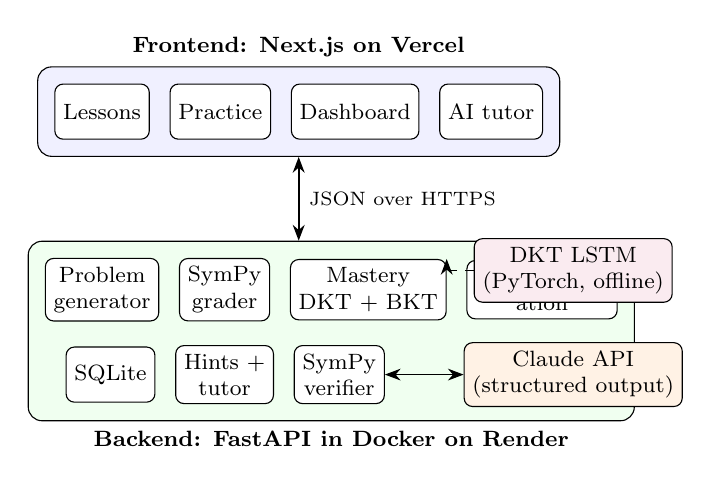
\begin{tikzpicture}[
  box/.style={draw, rounded corners=3pt, fill=white, align=center, font=\footnotesize, minimum height=7mm, inner sep=3pt},
  group/.style={draw, rounded corners=5pt, inner sep=6pt, fill=#1},
  >={Stealth[length=2mm]}]
  \node[box] (lesson) {Lessons};
  \node[box, right=2.5mm of lesson] (practice) {Practice};
  \node[box, right=2.5mm of practice] (dash) {Dashboard};
  \node[box, right=2.5mm of dash] (tutor) {AI tutor};
  \begin{scope}[on background layer]
    \node[group=blue!6, fit=(lesson)(tutor), label={[font=\footnotesize\bfseries]above:{Frontend: Next.js on Vercel}}] (fe) {};
  \end{scope}
  \node[box, below=15mm of lesson] (gen) {Problem\\generator};
  \node[box, right=2.5mm of gen] (grader) {SymPy\\grader};
  \node[box, right=2.5mm of grader] (kt) {Mastery\\DKT + BKT};
  \node[box, right=2.5mm of kt] (rec) {Recommend-\\ation};
  \node[box, below=3mm of grader] (hint) {Hints +\\tutor};
  \node[box, right=2.5mm of hint] (ver) {SymPy\\verifier};
  \node[box, left=2.5mm of hint] (db) {SQLite};
  \begin{scope}[on background layer]
    \node[group=green!6, fit=(gen)(rec)(hint)(db), label={[font=\footnotesize\bfseries]below:{Backend: FastAPI in Docker on Render}}] (be) {};
  \end{scope}
  \node[box, right=10mm of ver, fill=orange!10] (llm) {Claude API\\(structured output)};
  \node[box, above=5mm of llm, fill=purple!8] (dkt) {DKT LSTM\\(PyTorch, offline)};
  \draw[<->, thick] (fe.south) -- node[right, font=\scriptsize]{JSON over HTTPS} (fe.south |- be.north);
  \draw[<->] (ver.east) -- (llm.west);
  \draw[->, dashed] (dkt.west) -- (kt.east |- dkt.west) -- (kt.north east);
\end{tikzpicture}
\caption{Architecture. Every math step proposed by the LLM passes the SymPy verifier before reaching the browser.}
\label{fig:arch}
\end{figure}

Figure~\ref{fig:arch} shows the architecture: a Next.js frontend, a FastAPI backend with SQLite, a PyTorch DKT model trained offline, SymPy for grading and verification, and Claude for language, requested as structured JSON.

\paragraph{Curriculum.} Three courses (Pre-Algebra, Algebra~1, Algebra~2) contain 8 units and 18 topics: integers, exponents and roots, algebraic expressions, one- and multi-step linear equations, linear inequalities, polynomials and quadratic equations. Prerequisites form a directed acyclic graph. Each topic has a lesson with the idea, steps, a worked example and a common mistake; every line of every worked example is checked with SymPy in the test suite.

\paragraph{Problems and grading.} Template generators build each problem ``answer first'', so answers are integers and a problem is fully determined by \code{skill:seed}. The server regenerates problems from their id to grade them and never sends answers to the browser. The grader accepts any equivalent form (or solution set, for quadratics and inequalities), judges simplest form on the unevaluated parse ($x=8/2$ is ``right value, not simplified''), and gives targeted feedback such as ``check the direction of the inequality sign''. Because SymPy's parser uses \code{eval}, input is restricted to a character whitelist and a length cap, with small, non-chained exponents.

\paragraph{Mastery and recommendation.} DKT was trained on ASSISTments skills, so each topic is mapped to ASSISTments skills that have at least 1{,}000 training rows (enforced by a test), and a topic's mastery is DKT's mean predicted probability of a correct answer over those skills. Inequalities, polynomials and quadratics have essentially no ASSISTments data, so those 7 topics use BKT with hand-set parameters (prior 0.1, learn 0.1, guess 0.25, slip 0.1). Only a problem's first graded attempt updates mastery, and asking for a hint before answering counts as incorrect. The system recommends the lowest-mastery topic whose prerequisites are all mastered ($\geq 0.7$).

\paragraph{Verified hints.} Claude returns \code{\{hint, next\_step\}}. Before a student sees it, \code{next\_step} must parse, have the same solution set as the student's current step, make progress (judged on the written form, since distributing changes form but not value), and not be the final answer; the hint text is also scanned for the answer. Rejected hints are retried with the reasons, up to three attempts, and then replaced by a fixed, safe hint.

\paragraph{AI tutor.} A chat panel follows the student across the site: they can type a question, highlight any text, or ask for a unit to be explained. Replies include a walkthrough of \code{\{operation, result\}} steps that the frontend animates, highlighting added and removed terms and inequality sign flips (Figure~\ref{fig:screens}). Every step must have the same solution set as the starting line; true substitute-back checks such as $-7(8)+4=-52$ are allowed. When a practice problem is on screen, the tutor must use a similar problem instead, and replies that state the answer or use an example with the same solution are rejected. Unverifiable walkthroughs are dropped, and the tutor is rate-limited because each message costs API credit.

\begin{figure}[t]
\centering
\begin{subfigure}{0.49\linewidth}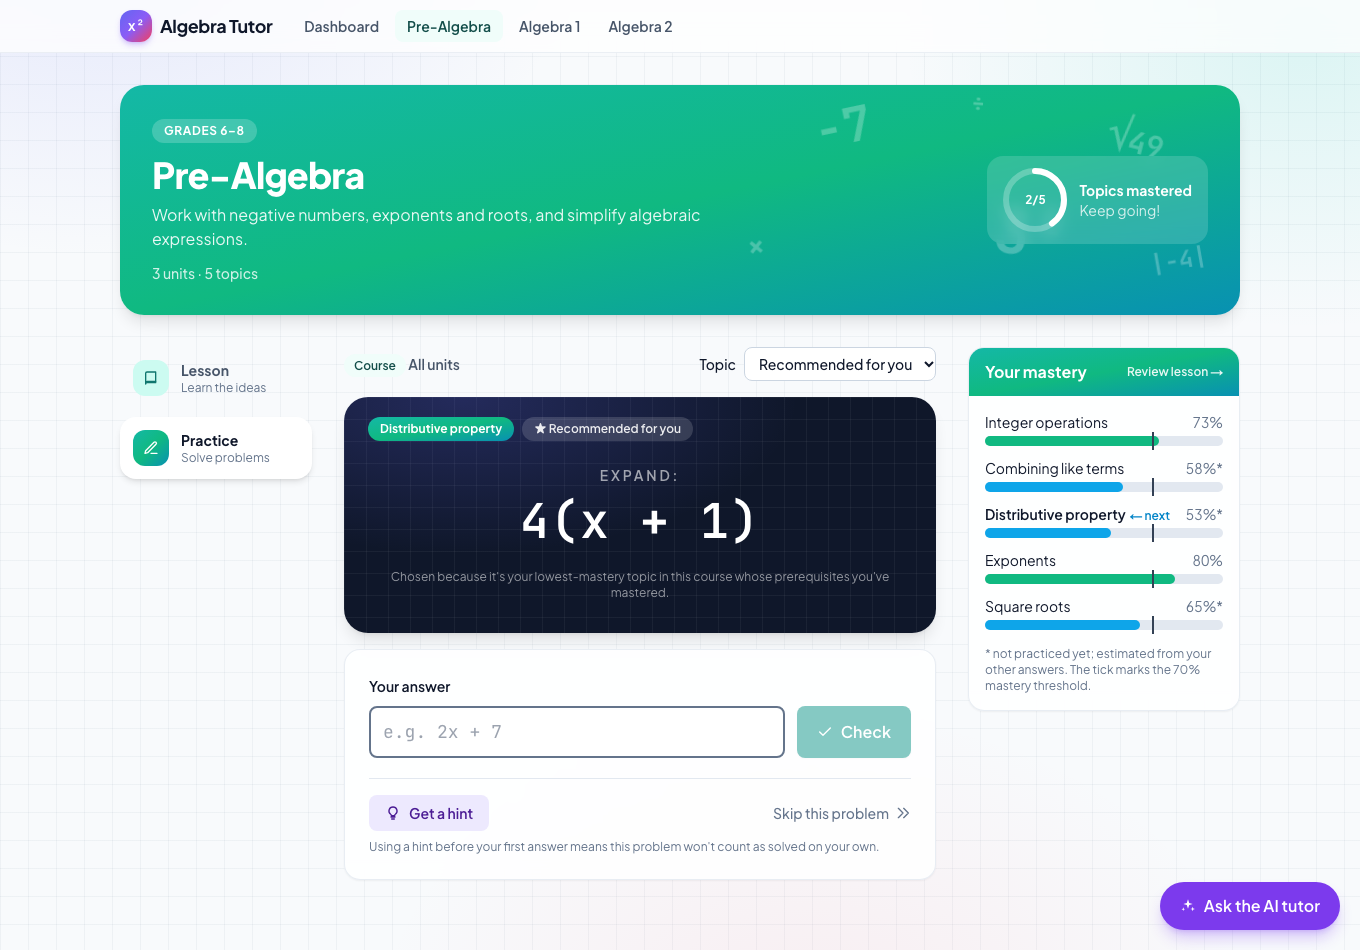
\includegraphics[width=\linewidth]{figures/practice.png}\caption{Practice with the mastery panel.}\end{subfigure}\hfill
\begin{subfigure}{0.49\linewidth}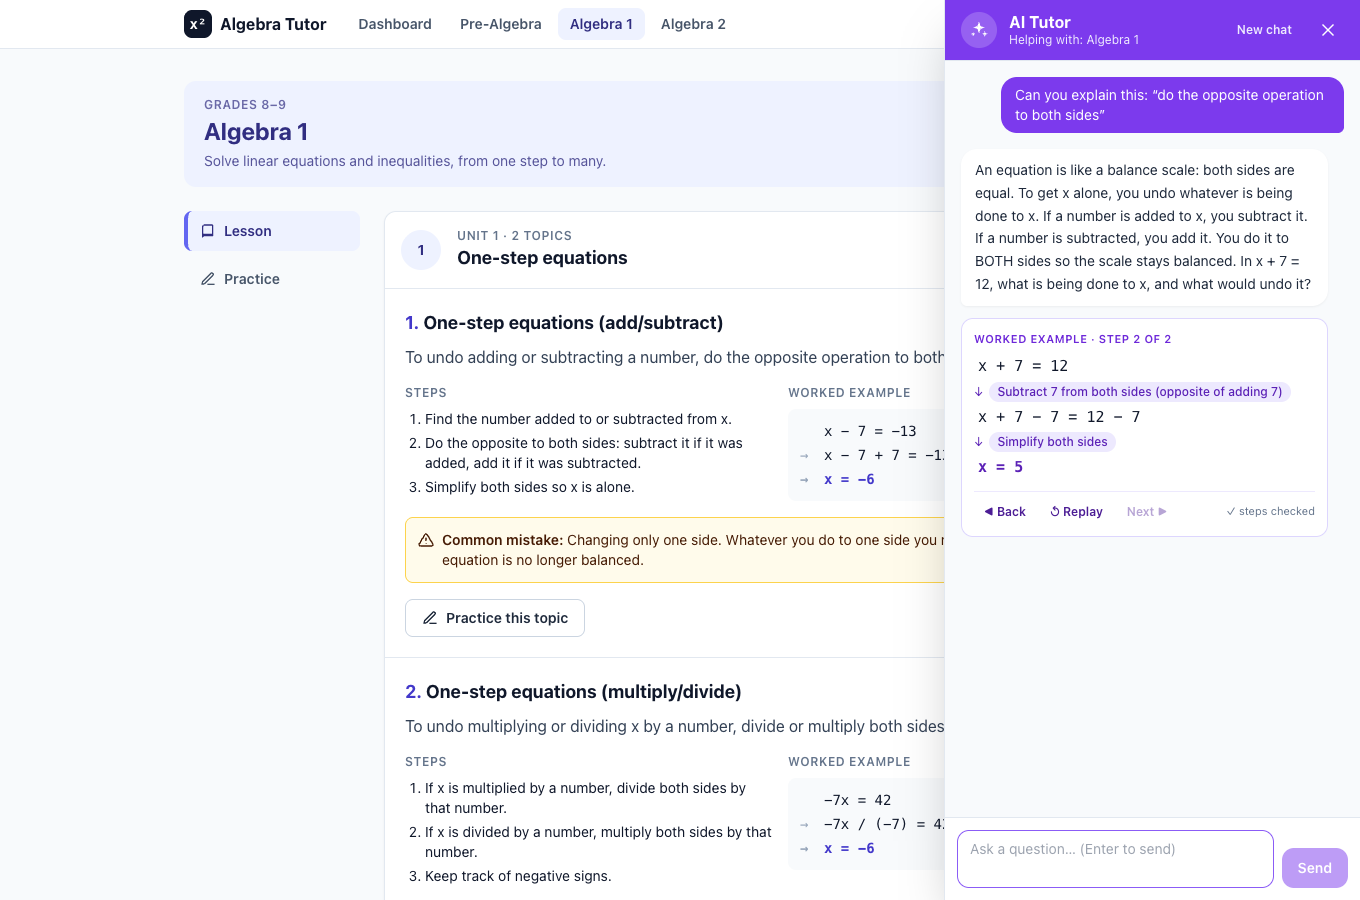
\includegraphics[width=\linewidth]{figures/tutor.png}\caption{AI tutor with a verified walkthrough.}\end{subfigure}
\caption{The deployed platform.}
\label{fig:screens}
\end{figure}

% ======================================================================
\section{Data}
We use the ASSISTments 2009--2010 skill-builder data~\cite{feng2009assistments}: 525{,}534 rows from 4{,}217 students. We drop rows without a skill, keep one row per answer (the raw file repeats an answer once per tagged skill, which would let a sequence model see the answer it is about to predict), and drop students with fewer than two answers, leaving 282{,}969 answers from 4{,}027 students on 112 skills. Students, not rows, are split 70/15/15 into training, validation and test sets (2{,}818 / 604 / 605 students), with all seeds fixed.

% ======================================================================
\section{Experiments}

\subsection{Experiment 1: DKT vs.\ BKT (RQ1)}
DKT embeds (skill, correct) tokens (size 100) into an LSTM (hidden size 100, dropout 0.2), trained with Adam (learning rate $10^{-3}$) with early stopping on validation AUC. BKT is pyBKT with one model per skill. Both predict every answer except each student's first and are scored identically. DKT improves test AUC by 0.043 (Table~\ref{tab:exp1}), consistent with its ability to share information across skills.

\begin{table}[ht]
\centering\small
\begin{tabular}{@{}lcccc@{}}
\toprule
Model & Val AUC & Val ACC & Test AUC & Test ACC \\
\midrule
BKT (pyBKT) & 0.716 & 0.721 & 0.708 & 0.708 \\
\textbf{DKT (LSTM)} & \textbf{0.755} & \textbf{0.739} & \textbf{0.751} & \textbf{0.731} \\
\bottomrule
\end{tabular}
\caption{Knowledge tracing (test set: 35{,}789 predictions).}
\label{tab:exp1}
\end{table}

\subsection{Experiment 2: Verified hints (RQ2)}
We made 127 hint requests across the 9 linear-equation skills, including each equation's real last step ($cx=d$), where leaking the answer is most tempting. The design is \emph{paired}: the LLM's first proposal is what an unverified system would show, and the final output is what students see. Leaks were flagged automatically and then audited by hand.

\begin{table}[ht]
\centering\small
\begin{tabular}{@{}llcccc@{}}
\toprule
Model & Condition & Math errors & Leaks (audited) & Wrong prose$^{*}$ & Calls/hint \\
\midrule
Claude Opus 5.5 & without check & 0\% & 0.8\% (1) & 0 & 1 \\
Claude Opus 5.5 & with check & 0\% & 0.8\% (1) & 0 & 1.0 \\
Claude Haiku 5.5 & without check & 0\% & 7.9\% (10) + 1 borderline & 2 & 1 \\
Claude Haiku 5.5 & with check & 0\% & \textbf{0\%} + 1 borderline & 2 & 1.11 \\
\bottomrule
\end{tabular}
\caption{Hint verification ($n=127$ per row). $^{*}$Only hints flagged by the broad leak measure were audited for wrong prose, so this is a lower bound.}
\label{tab:exp2}
\end{table}

Verification removed every detectable leak from the weaker model for 11\% more LLM calls, while the stronger model rarely needed it (Table~\ref{tab:exp2}). SymPy cannot check wording: Opus's single leak was in prose (``0 divided by any nonzero number is 0'' when $x=0$), and Haiku twice called a correct student step wrong. The experiment also exposed three bugs in our own pipeline (a progress check that rejected correct distribution steps, a leak check that read $8x=0$ as $x=0$, and unreachable test states); the invalid first run is kept in the log.

\subsection{Experiment 3: Verified tutor walkthroughs (RQ3)}
We made 40 paired tutor requests: for each of the 8 units, three ``explain this unit'' requests and two ``just tell me the answer'' requests with a practice problem on screen. All first replies contained a walkthrough; after one verifier fix (below), none had a math error or leaked the answer, and 100\% of shown walkthroughs were fully verified, at 1.05 LLM calls and 3.4\,s per request (\$0.45 in total). The first run reported 5\% ``math errors'', but both were correct substitute-back checks that our verifier wrongly rejected. A verifier's false positives also cost pedagogical quality, so the verifier itself must be tested.

% ======================================================================
\section{Discussion}
\paragraph{Engineering.} 291 automated tests cover the grader (including malicious inputs), the generators (300 seeds per skill, each verified by SymPy), every worked-example line, recommendation, BKT, mastery routing, hints, the tutor and the API. Every experiment is logged with its raw outputs. The system is deployed with Docker on Render and Next.js on Vercel, and an automated browser walkthrough tests the live site.

\paragraph{Limitations.} (1)~Topics are mapped to ASSISTments skills by hand, and several topics share one skill, so their mastery estimates move together. (2)~BKT parameters for the 7 topics without data are hand-set. (3)~Verification covers mathematics, not language, so misleading wording can pass. (4)~We did not measure learning gains with real students. (5)~The LLM experiments are small (127 hints and 40 tutor requests) and the audit used a single annotator. (6)~The free hosting tier resets the database on restart.

\paragraph{Future work.} A classroom study of learning gains; knowledge tracing data for Algebra~2 topics, or BKT parameters fitted from the platform's own logs; verifying equations inside the explanation text; and attention-based knowledge tracing~\cite{pandey2019sakt}.

\section{Conclusion}
\todo{3--5 sentences in your own words: what you built, the answer to each research question, and the main lesson. Suggested lesson: LLMs are useful tutors when their mathematical claims are verified, but the verifier itself must be tested, because both its misses and its false alarms affect students.}

\section*{Reflection}
\todo{A short paragraph in your own words: what was hardest, what you would do differently, and why you changed the scope (course platform, AI tutor).}

\medskip
\noindent\small Live site: \url{https://ai-algebra-tutor-pi.vercel.app}

\bibliographystyle{plainnat}
\bibliography{references}

\end{document}
